%%%%%%%%%%%%%%%%%%%%%%%%%%%%%%%%%%%%%%%%%%%%%%%%%%%%%%%%%%%%%%%%%
%%% %
%%% % weiiszablon.tex
%%% % The Faculty of Electrical and Computer Engineering
%%% % Rzeszow University Of Technology diploma thesis Template
%%% % Szablon pracy dyplomowej Wydziału Elektrotechniki 
%%% % i Informatyki PRz
%%% % January, 2024
%%%%%%%%%%%%%%%%%%%%%%%%%%%%%%%%%%%%%%%%%%%%%%%%%%%%%%%%%%%%%%%%%

\documentclass[12pt,twoside]{article}

\usepackage{weiiszablon}
\usepackage{float}
\author{Dawid Kurzępa 179946}

% np. EF-123456, EN-654321, ...
\studentID{179946}

\title{Dla zadanego ciągu liczb naturalnych, znajdź długość
najkrótszego ciągu, którego suma jest większa niż zadana
liczba. }
\titleEN{For a given sequence of natural numbers, find the length of
the shortest sequence whose sum is greater than the specified value
number.}


%%% wybierz rodzaj pracy wpisując jeden z poniższych numerów: ...
% 1 = inżynierska	% BSc
% 2 = magisterska	% MSc
% 3 = doktorska		% PhD
% 4 = praca inżynierska
%%% na miejsce zera w linijce poniżej
\newcommand{\rodzajPracyNo}{5} 
%Pozwoliłem sobie dopisać 5 rodzaj pracy, zadanie programistyczne


%%% promotor
\supervisor{dr inż. Mariusz Borkowski prof. PRz}
%% przykład: dr hab. inż. Józef Nowak, prof. PRz

%%% promotor ze stopniami naukowymi po angielsku
\supervisorEN{Prof. Imię i nazwisko opiekuna, (academic degree)}

\abstract{W pracy zaprezentowano trzy metody znajdowania najkrótszego podciągu liczb naturalnych, którego suma przekracza zadaną wartość: sortowanie i wybór największych elementów, algorytm sliding window oraz podejście dynamiczne. Porównano ich efektywność oraz złożoność obliczeniową, przedstawiając wykresy i schematy blokowe. Implementacja została wykonana w C++.}
\abstractEN{This paper presents three methods for finding the shortest subsequence of natural numbers whose sum exceeds a given value: sorting and selecting the largest elements, the sliding window algorithm, and a dynamic approach. Their efficiency and complexity were compared using graphs and flowcharts. The implementation was done in C++.}

\keywords{C++, podciągi, algorytmy, analiza złożoności, schematy blokowe}
\keywordsEN{C++, subsequences, algorithms, complexity analysis, flowcharts}


\begin{document}

% strona tytułowa
\maketitle

\blankpage

% spis treści
\tableofcontents

\clearpage
\blankpage


\section{Wstęp}

\subsection{Cel}
Celem zadania jest opracowanie, implementacja oraz analiza algorytmów znajdujących najkrótszy podciąg, którego suma jest większa niż zadana liczba.

\subsection{Zakres problemu}
Zadanie obejmuje trzy podejścia algorytmiczne rozwiązujące zadany problem oraz ich analizę.

\subsection{Omówienie metod}
W pracy wykorzystano trzy metody rozwiązania problemu :
Sortowanie i sumowanie największych liczb,
Sliding Window (okno przesuwne),
Dynamic Programming (brute-force optymalizowane)

\section{Opis problemu}

\subsection{Przedstawienie problemu}
Dla danego ciągu liczb naturalnych oraz liczby, należy znaleźć najkrótszy ciąg liczb z tego zbioru, którego suma jest większa niż zadana liczba k.

\subsection{Dane wejściowe i wyjściowe}
Dane wejściowe: Ciąg liczb naturalnych oraz liczba k.\\
Dane wyjściowe: Najkrótszy ciąg liczb, którego suma jest większa niż liczba k.

\subsection{Przykładowe dane i oczekiwany wynik}
Wejście: \{1, 2, 3, 4, 5, 6, 7, 8\}, k = 20, – Wyjście: \{6, 7, 8\}\\
Wejście: \{1, 2, 3, 4, 5, 6, 7, 8\}, k = 7, – Wyjście: \{8\}\\
Wejście: \{1, 2, 3, 4, 5, 6, 7, 8\}, k = 21, – Wyjście: \{5, 6, 7, 8\}\\
wejście: \{1,2,3,4,5,6,7,8\}, k = 40, - Wyjście: Brak odpowiedniego podciągu!

\section{Podejścia do rozwiązania problemu}

\subsection{Sortowanie i sumowanie największych liczb}

\subsubsection{Opis podejścia}
Metoda Sortowanie i sumowanie największych liczb polega na posortowaniu ciągu liczb w kolejności malejącej, a następnie sumowaniu największych elementów, aż suma przekroczy zadaną wartość. Po znalezieniu takiego podciągu, algorytm zwraca jego długość jako rozwiązanie. To podejście jest proste do zaimplementowania, ale wymaga sortowania, co wpływa na jego złożoność obliczeniową.

\subsubsection{Podstawy teoretyczne}
Liczba wszystkich podciągów dla ciągu o długości \( n \) wynosi:

\begin{equation}
    2^n
    \label{eq:liczba_podciagow}
\end{equation}
Metoda sortuje liczby za pomocą algorytmu \textbf{Bubble Sort} i sumuje największe, aż przekroczy zadaną wartość. Dzięki temu ogranicza liczbę sprawdzanych elementów, osiągając złożoność \( O(n^2) \) przez użycie algorytmu Bubble Sort.

\subsubsection{Złożoność czasowa i obliczeniowa}
\textbf{Złożoność czasowa:}
\begin{itemize}
    \item \textbf{Sortowanie (Bubble Sort):} Bubble sort ma złożoność czasową $O(n^2)$, ponieważ dla każdego elementu porównuje się go z innymi elementami w tablicy w najgorszym przypadku.
    \item \textbf{Iteracja przez posortowaną listę:} Po posortowaniu listy, iteracja przez elementy listy w celu znalezienia najkrótszego podciągu ma złożoność $O(n)$.
\end{itemize}
\textbf{Złożoność całkowita:}
\begin{itemize}
    \item \textbf{Złożoność czasowa:} $O(n^2)$ (dominująca część to sortowanie)
    \item \textbf{Złożoność pamięciowa:} $O(n)$, ponieważ potrzebujemy tylko jednej dodatkowej zmiennej do przechowywania sumy i długości podciągu (pomijając samą tablicę liczb).
\end{itemize}
\subsubsection{Wady i zalety}

\textbf{Zalety:}
\begin{itemize}
    \item Prosta koncepcja – metoda polega na posortowaniu liczb i sumowaniu największych z nich, co jest łatwe do zrozumienia.
    \item Łatwość implementacji – w porównaniu do bardziej skomplikowanych algorytmów, metoda sortowania i sumowania jest stosunkowo łatwa do zaimplementowania.
\end{itemize}
\textbf{Wady:}
\begin{itemize}
    \item Złożoność czasowa w zależności od algorytmu sortowania – jeśli użyjemy algorytmu o złożoności $O(n^2)$, jak bubble sort, cała metoda będzie miała złożoność $O(n^2)$.
    \item Może być nieoptymalna, gdy dane wejściowe są już posortowane lub gdy mamy do czynienia z dużymi zestawami danych.
    \item Sortowanie w celu znalezienia najkrótszego podciągu może być zbędne, jeśli wystarczyłaby inna metoda optymalizacyjna.
\end{itemize}

\subsubsection{Implementacja w pseudokodzie}

\begin{itemize}
  \item Funkcja FindShortestSubsequence:
  \item Wejście: lista liczb, k
  \item Posortuj listę liczb w porządku malejącym
  \item Inicjalizuj sumę na 0
  \item Inicjalizuj zmienną dla długości podciągu
  \item Dla każdego elementu w posortowanej liście:
  \begin{itemize}
      \item Dodaj element do sumy
      \item Zwiększ długość podciągu
      \item Jeśli suma > k, zakończ
  \end{itemize}
  \item Jeśli nie znaleziono odpowiedniego podciągu:
  \item Zwróć komunikat o braku rozwiązania
  \item Zwróć długość podciągu
\end{itemize}

\subsubsection{Implementacja w schemacie blokowym}

\begin{figure}
    \centering
    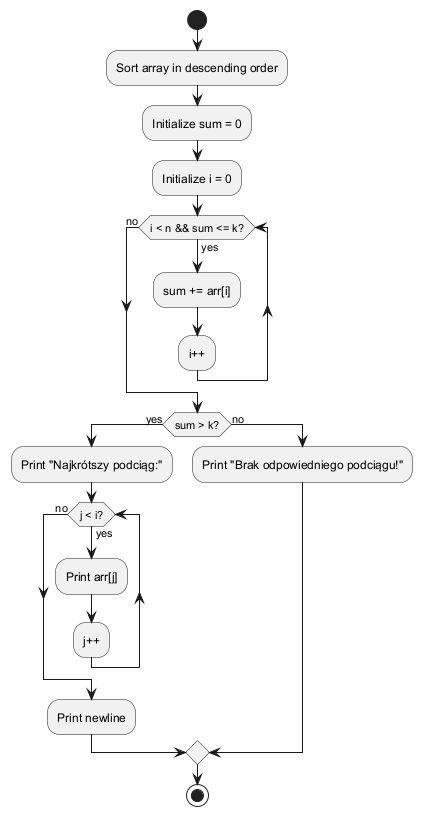
\includegraphics[width=0.50\linewidth]{schemat1.png}
    \caption{schemat blokowy Sortowanie i Sumowanie}
\end{figure}
\clearpage
\subsection{Sliding Window (okno przesuwne)}
\subsubsection{Opis podejścia}

Metoda okna przesuwnego (sliding window) polega na iteracyjnym sprawdzaniu podciągów o rosnącym rozmiarze w danej tablicy, gdzie "okno" przesuwa się po elementach w sposób ciągły. Początkowo okno obejmuje początkowe elementy, a następnie stopniowo rozszerza się lub przesuwa, aż spełni warunki zadania. Jest to efektywna metoda o złożoności czasowej $O(n)$, idealna do rozwiązywania problemów z ciągłymi fragmentami danych.

\subsubsection{Podstawy teoretyczne}

Metoda okna przesuwnego jest techniką wykorzystywaną do rozwiązywania problemów związanych z przetwarzaniem ciągów danych w sposób efektywny. Główna idea polega na tym, że rozpatrujemy tylko część ciągu, zwaną "oknem", i przesuwamy to okno po ciągu, przy czym w każdym kroku obliczamy wynik dla bieżącego podciągu. Okno ma zazwyczaj stałą wielkość, ale może się zmieniać w zależności od wymagań problemu.

Jeśli mamy ciąg liczb o długości $n$, to metoda okna przesuwnego pozwala na rozwiązywanie problemów, takich jak znajdowanie największej sumy podciągu o zadanej długości, bez konieczności ponownego przetwarzania całego ciągu w każdym kroku. Działanie algorytmu polega na dodaniu nowego elementu do okna i usunięciu elementu, który wychodzi poza zakres okna. Dzięki temu, operacje są wykonywane w czasie $O(1)$ w każdym kroku, a cała złożoność czasowa algorytmu wynosi $O(n)$.

Metoda okna przesuwnego jest szczególnie użyteczna w problemach, gdzie trzeba obliczać wynik dla wielu podciągów ciągu w sposób efektywny, bez konieczności rozważania każdego możliwego podciągu.

\subsubsection{Złożoność czasowa i obliczeniowa}

Złożoność czasowa metody okna przesuwnego wynosi $O(n)$, gdzie $n$ to liczba elementów w ciągu danych wejściowych. Jest to możliwe dzięki temu, że w każdym kroku operacje związane z dodaniem nowego elementu do okna i usunięciem elementu wychodzącego z okna wykonują się w czasie stałym $O(1)$. W rezultacie cała metoda wymaga tylko jednego przejścia przez dane wejściowe.

Złożoność obliczeniowa tej metody jest bardzo efektywna, ponieważ jej zapotrzebowanie na pamięć wynosi $O(1)$, co oznacza, że nie potrzebujemy dodatkowych struktur danych o rozmiarze zależnym od wielkości wejścia. Okno przesuwne przetwarza dane w sposób ciągły, zmieniając tylko kilka zmiennych pomocniczych, co zapewnia minimalne zużycie pamięci.

\subsubsection{Wady i zalety}

\textbf{Zalety:}
\begin{itemize}
    \item Złożoność czasowa $O(n)$ – bardzo szybka metoda, działająca w czasie liniowym.
    \item Złożoność pamięciowa $O(1)$ – minimalne zużycie pamięci, ponieważ wykorzystujemy tylko kilka zmiennych pomocniczych.
    \item Efektywna przy problemach wymagających ciągłych obliczeń dla fragmentów danych.
\end{itemize}
\textbf{Wady:}
\begin{itemize}
    \item Wymaga przetworzenia danych w sposób iteracyjny, co może być trudne do zaimplementowania w porównaniu do prostszych algorytmów.
    \item Działa głównie na problemach, w których okno ma stałą lub zmieniającą się wielkość, co może ograniczać zastosowanie w bardziej złożonych przypadkach.
\end{itemize}

\subsubsection{Implementacja w pseudokodzie}
\begin{itemize}
  \item Funkcja FindShortestSubsequence:
  \item Wejście: lista liczb, k
  \item Inicjalizuj sumę jako 0
  \item Inicjalizuj minimalną długość podciągu jako nieskończoność
  \item Inicjalizuj indeks początkowy podciągu (lewy) jako 0
  \item Dla każdego elementu (prawy) w liście:
  \begin{itemize}
      \item Dodaj bieżący element do sumy
      \item Dopóki suma jest większa niż k:
      \begin{itemize}
          \item Zaktualizuj minimalną długość podciągu
          \item Odejmij element na pozycji lewy od sumy
          \item Zwiększ wartość lewy
      \end{itemize}
  \end{itemize}
  \item Jeśli nie znaleziono odpowiedniego podciągu:
  \item Zwróć komunikat o braku rozwiązania
  \item W przeciwnym razie zwróć minimalną długość podciągu
\end{itemize}
\subsubsection{Implementacja w schemacie blokowym}

\clearpage
\begin{figure}
    \centering
    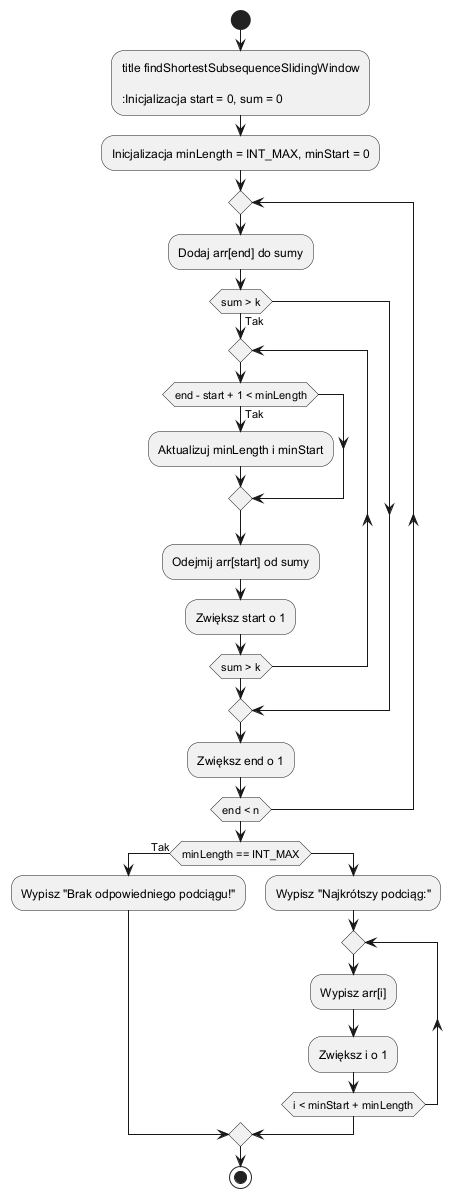
\includegraphics[width=0.5\linewidth]{schemat2.png}
    \caption{schemat blokowy Okno przesuwne}
    \label{fig:enter-label}
\end{figure}
\clearpage
\subsection{Metoda brute-force optymalizowane}

\subsubsection{Opis podejścia}
Metoda brute-force optymalizowane opiera się na sprawdzeniu wszystkich możliwych podciągów w sposób systematyczny, ale z wykorzystaniem optymalizacji przyspieszających działanie algorytmu. Zamiast sprawdzać każdy podciąg niezależnie, algorytm eliminuje niepotrzebne obliczenia, np. przerywa iterację, gdy suma podciągu przekroczy wartość progową.

\subsubsection{Podstawy teoretyczne}
W najgorszym przypadku liczba wszystkich podciągów w ciągu o długości $n$ wynosi:
\begin{equation}
    \sum_{i=1}^{n} i = \frac{n(n+1)}{2}
    \label{eq:suma_podciagow}
\end{equation}
Dzięki zastosowaniu optymalizacji, takich jak wcześniejsze zakończenie przetwarzania, rzeczywista liczba analizowanych podciągów jest mniejsza, co poprawia wydajność w porównaniu do klasycznej metody brute-force.

\subsubsection{Złożoność czasowa i obliczeniowa}
Podstawowa wersja brute-force ma złożoność czasową $O(n^2)$, jednak dzięki wczesnemu zakończeniu analizy niektórych podciągów rzeczywista wydajność jest lepsza w praktyce. Złożoność pamięciowa tej metody wynosi $O(1)$, ponieważ algorytm używa jedynie zmiennych pomocniczych do przechowywania sumy i długości podciągu.

\subsubsection{Wady i zalety}

\textbf{Zalety:}
\begin{itemize}
    \item Łatwiejsza implementacja w porównaniu do bardziej złożonych metod.
    \item Działa dla dowolnych danych wejściowych bez specjalnych założeń.
    \item Optymalizacja znacząco przyspiesza działanie w porównaniu do klasycznej wersji brute-force.
\end{itemize}

\textbf{Wady:}
\begin{itemize}
    \item Nadal gorsza wydajność niż metody oparte na oknie przesuwnym.
    \item W najgorszym przypadku nadal może wymagać sprawdzenia wszystkich podciągów.
\end{itemize}

\subsubsection{Implementacja w pseudokodzie}

\begin{itemize}
  \item Funkcja FindShortestSubsequence:
  \item Wejście: lista liczb, k
  \item Inicjalizuj minimalną długość podciągu jako nieskończoność
  \item Dla każdego indeksu początkowego w liście:
  \begin{itemize}
      \item Inicjalizuj sumę jako 0
      \item Dla każdego indeksu końcowego od punktu początkowego:
      \begin{itemize}
          \item Dodaj bieżący element do sumy
          \item Jeśli suma $> k$, zaktualizuj minimalną długość i przerwij pętlę
      \end{itemize}
  \end{itemize}
  \item Jeśli nie znaleziono odpowiedniego podciągu:
  \item Zwróć komunikat o braku rozwiązania
  \item W przeciwnym razie zwróć minimalną długość podciągu
\end{itemize}
\subsubsection{Implementacja w schemacie blokowym}
\clearpage
\begin{figure}
    \centering
    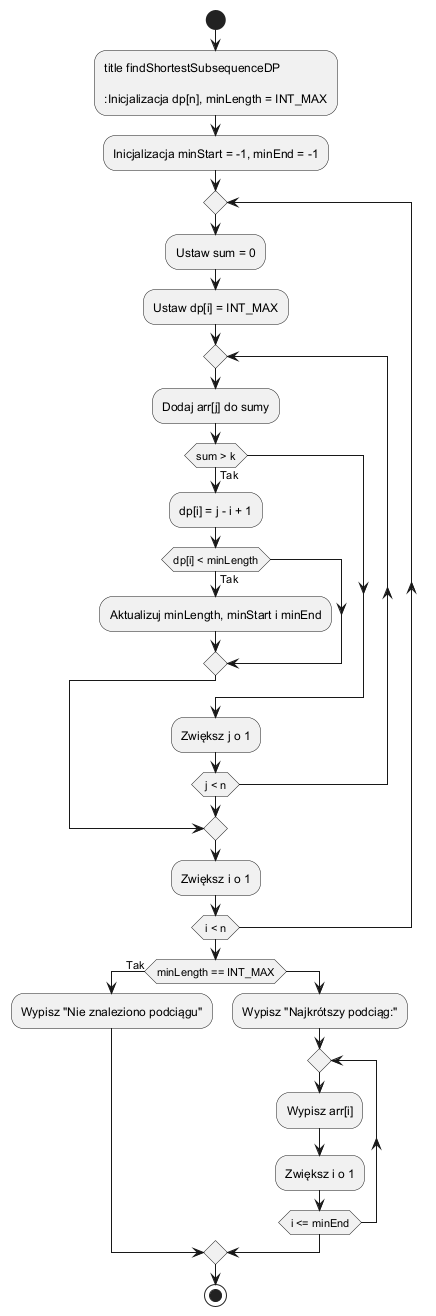
\includegraphics[width=0.5\linewidth]{schemat3.png}
    \caption{Schemat blokowy Brute force}
    \label{fig:enter-label}
\end{figure}

\section{Wyniki testów i wykres czasu}
\subsection{Wyniki testów czasowych}
Przykładowy wynik dla tablicy 1-n dla n = 10000 oraz k = 500000
\subsubsection{Sortowanie i sumowanie}

\begin{figure}[!h]
    \centering
    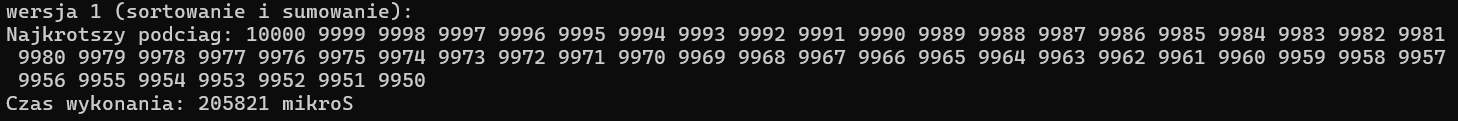
\includegraphics[width=1\linewidth]{czas1.png}
    \caption{pomiar czasu sortowanie sumowanie}
    \label{fig:enter-label}
\end{figure}

\subsubsection{Okno przesuwne}

\begin{figure}[!h]
    \centering
    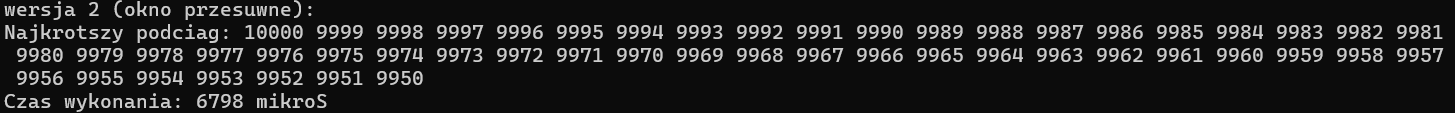
\includegraphics[width=1\linewidth]{czas2.png}
    \caption{pomiar czasu okno przesuwne}
    \label{fig:enter-label}
\end{figure}

\subsubsection{Brute force}

\begin{figure}[!h]
    \centering
    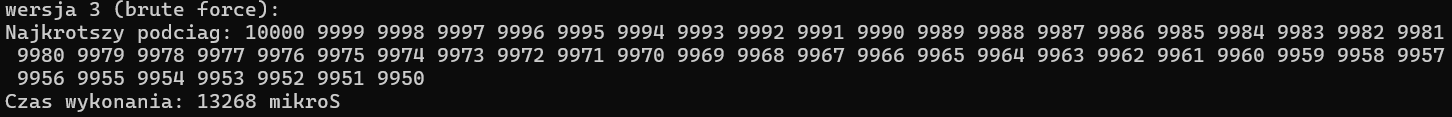
\includegraphics[width=1\linewidth]{czas3.png}
    \caption{pomiar czasu brute force}
    \label{fig:enter-label}
\end{figure}

\subsection{Wykresy czasu obliczeniowego}

\subsubsection{Sortowanie i sumowanie}

\begin{figure}[!h]
    \centering
    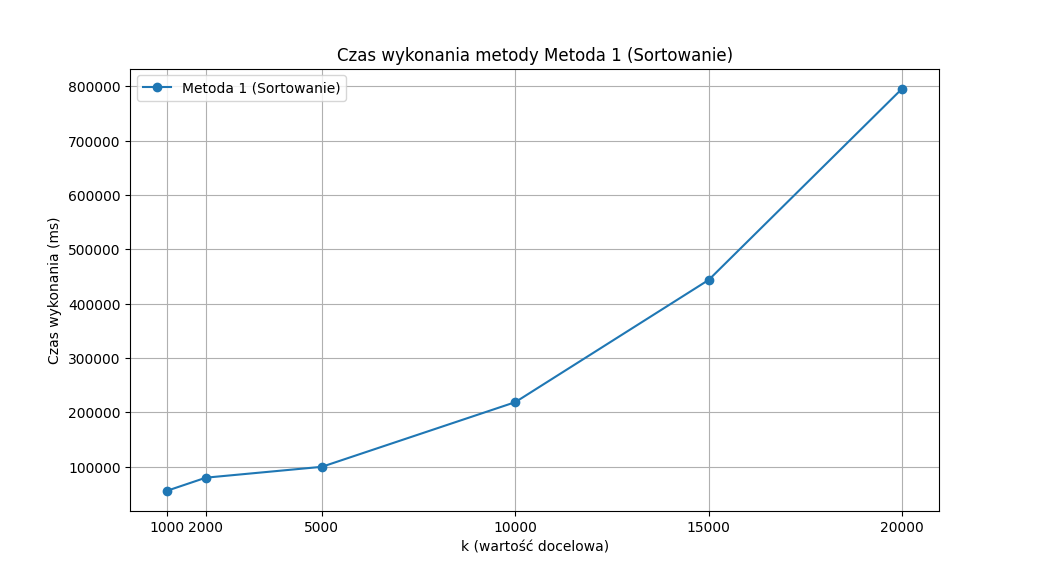
\includegraphics[width=1\linewidth]{wykres_1.png}
    \caption{Wykres czasu sortowanie i sumowanie}
    \label{fig:enter-label}
\end{figure}
\clearpage
\subsubsection{Okno przesuwne}

\begin{figure}[!h]
    \centering
    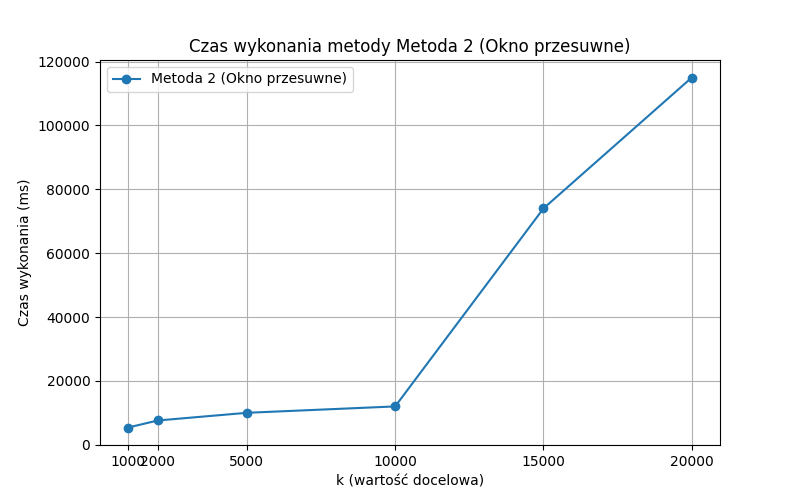
\includegraphics[width=1\linewidth]{wykres_2.png}
    \caption{Wykres czasu okno przesuwne}
    \label{fig:enter-label}
\end{figure}
\clearpage
\subsubsection{Brute force}

\begin{figure}[!h]
    \centering
    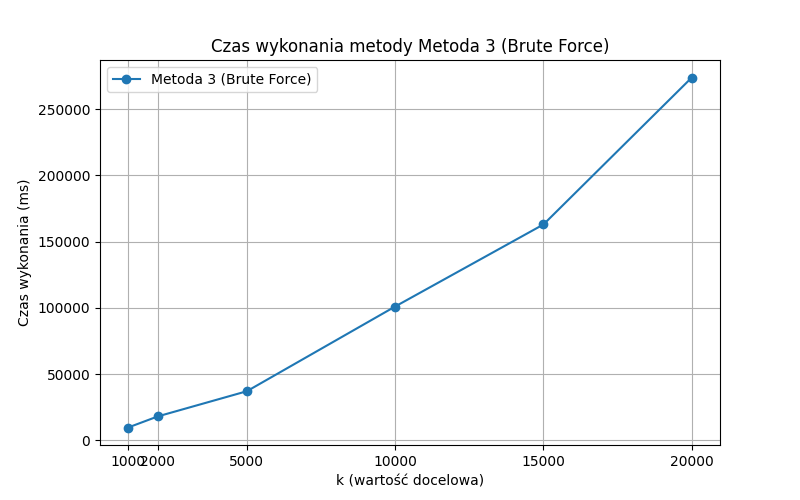
\includegraphics[width=1\linewidth]{wykres_3.png}
    \caption{Wykres czasu brute force}
    \label{fig:enter-label}
\end{figure}
\clearpage

\section{Wnioski i podsumowanie}
\begin{itemize}
    \item Analizując wykresy z przeprowadzonych badań dla dobranych zakresów wartości widać, że sortowanie wypada najsłabiej niezależnie od wielkości tablicy - nawet jeśli różnice są niewielkie.
    \item Okno przesuwne sprawdza się najlepiej dla każdych testowanych liczb ze znaczną przewagą
    \item Metoda brute force jest uśrednieniem czasu potrzebnego do wykonania zadania względem poprzednich prób
\end{itemize}
\section{Załączniki}
\addcontentsline{toc}{section}{Materiały}
\centering
\begin{lstlisting}[language=C++, caption={main.cpp}, label={lst:program}]
#include <iostream>
#include <windows.h> 	
#include <chrono>
using namespace std;
using namespace std::chrono;

// bubble sort O(n^2)	
void sortDescending(int arr[], int n) { 
    for (int i = 0; i < n - 1; i++) {
        for (int j = 0; j < n - i - 1; j++) {
            if (arr[j] < arr[j + 1]) {
                int temp = arr[j];
                arr[j] = arr[j + 1];
                arr[j + 1] = temp;
            }
        }
    }
}

// Funkcja znajdująca najkrótszy podciąg o sumie większej niż k
void findShortestSubsequence(int arr[], int n, int k) { // cała funkcja ma złożoność O(n^2) przez sortowanie, gdyby zastosować quicksort O(n log n)
    // Wywołanie funkcji sortującej tablicę w porządku malejącym
    sortDescending(arr, n); // Funkcja sortująca tablicę arr o długości n w porządku malejącym

    // Inicjalizacja zmiennych pomocniczych
    int sum = 0; // Zmienna do przechowywania sumy elementów w podciągu
    int i = 0;   // Indeks, który będzie wskazywał liczbę elementów w najkrótszym podciągu

    // Szukamy najkrótszego podciągu o sumie większej niż k
    // Pętla przetwarza tablicę i sumuje elementy, dopóki suma nie przekroczy k
    while (i < n && sum <= k) {
        sum += arr[i]; // Dodajemy element z tablicy do sumy
        i++; // Przechodzimy do kolejnego elementu tablicy
    }

    // Sprawdzamy, czy znaleziono podciąg
    if (sum > k) {
        // Jeśli suma jest większa niż k, wypisujemy najkrótszy podciąg
        cout << "Najkrotszy podciag: ";
        for (int j = 0; j < i; j++) {  // Wypisujemy elementy podciągu
            cout << arr[j] << " "; // Wypisujemy element na pozycji j
        }
        cout << endl; // Koniec wypisywania
    } else {
        // Jeśli suma nigdy nie przekroczyła k
        cout << "Brak odpowiedniego podciagu!"<< endl;
    }
}

void findShortestSubsequenceSlidingWindow(int arr[], int n, int k) { // cała funkcja ma złożoność O(n) - każdy element jest przetwarzany maksymalnie raz
    // Inicjalizacja zmiennych pomocniczych
    int start = 0, sum = 0, minLength = INT_MAX, minStart = 0;
    // 'start' wskazuje początek okna, 'sum' to suma elementów w oknie
    // 'minLength' to długość najkrótszego podciągu, który spełnia warunek, domyślnie maksymalna wartość typu int
    // 'minStart' to indeks początkowy tego podciągu

    // Przesuwanie okna po tablicy
    for (int end = 0; end < n; end++) {
        sum += arr[end]; // Dodajemy element z pozycji 'end' do sumy okna

        // Zmniejszamy okno, gdy suma przekroczy wartość k
        while (sum > k) {
            // Sprawdzamy, czy obecne okno jest najkrótszym, które spełnia warunek
            if (end - start + 1 < minLength) {
                minLength = end - start + 1; // Aktualizujemy długość najkrótszego podciągu
                minStart = start; // Zapamiętujemy początek tego podciągu
            }

            // Usuwamy element od początku okna (przesuwamy wskaźnik 'start' w prawo)
            sum -= arr[start]; // Odejmujemy element, który zostaje usunięty z okna
            start++; // Przesuwamy początek okna w prawo
        }
    }

    // Sprawdzamy, czy znaleziono jakikolwiek podciąg
    if (minLength == INT_MAX) {
        // Jeśli długość pozostała maksymalna, to znaczy, że nie znaleziono podciągu
        cout << "Brak odpowiedniego podciagu!" << endl;
    } else {
        // Wypisujemy najkrótszy podciąg
        cout << "Najkrotszy podciag: ";
        for (int i = minStart; i < minStart + minLength; i++) {
            cout << arr[i] << " "; // Wypisujemy elementy najkrótszego podciągu
        }
        cout << endl; // Koniec wypisywania
    }
}


void findShortestSubsequenceDP(int arr[], int n, int k) { // w najgorszym przypadku O(n^2)
    // Tablica do przechowywania minimalnej długości podciągu dla danego indeksu
    int dp[n];  
    int minLength = INT_MAX; // Przechowuje globalną minimalną długość podciągu spełniającego warunek
    int minStart = -1, minEnd = -1; // Indeksy początku i końca znalezionego podciągu

    // Przechodzimy przez wszystkie indeksy i obliczamy najkrótszy podciąg
    for (int i = 0; i < n; i++) {
        int sum = 0; // Resetujemy sumę dla każdego indeksu
        dp[i] = INT_MAX; // Początkowo zakładamy, że nie ma podciągu

        for (int j = i; j < n; j++) {
            sum += arr[j]; // Dodajemy kolejne liczby do sumy

            if (sum > k) { // Jeśli suma przekroczyła k
                dp[i] = j - i + 1; // Długość podciągu to różnica indeksów + 1
                
                // Sprawdzamy, czy znaleziony podciąg jest krótszy niż poprzednie
                if (dp[i] < minLength) {
                    minLength = dp[i];
                    minStart = i;
                    minEnd = j;
                }
                break; // Przerywamy, bo znaleźliśmy minimalny podciąg dla tego i
            }
        }
    }

    // Wypisywanie wyniku
    if (minLength == INT_MAX) {
        cout << "Nie znaleziono podciagu, ktorego suma jest większa niz " << k << endl;
    } else {
        cout << "Najkrotszy podciag: ";
        for (int i = minStart; i <= minEnd; i++) {
            cout << arr[i] << " ";
        }
        cout << endl;
    }
}

int main() {
    // Tworzenie tablicy liczb od 1 do SIZE
    const int SIZE = 10000; // n
    int numbers[SIZE];
    for (int i = 0; i < SIZE; i++) {
        numbers[i] = i + 1;
    }

    int k = 3000;  // liczba do przewazenia podciagiem

    // Pomiar czasu dla wersji 1
    cout << "wersja 1 (sortowanie i sumowanie):" << endl;
    auto start1 = high_resolution_clock::now();
    findShortestSubsequence(numbers, SIZE, k);
    auto stop1 = high_resolution_clock::now();
    auto duration1 = duration_cast<microseconds>(stop1 - start1);
    cout << "Czas wykonania: " << duration1.count() << " mikroS\n" << endl; //1 sekunda = 1 000 000 mikrosekund

    // Pomiar czasu dla wersji 2
    cout << "wersja 2 (okno przesuwne):" << endl;
    auto start2 = high_resolution_clock::now();
    findShortestSubsequenceSlidingWindow(numbers, SIZE, k);
    auto stop2 = high_resolution_clock::now();
    auto duration2 = duration_cast<microseconds>(stop2 - start2);
    cout << "Czas wykonania: " << duration2.count() << " mikroS\n" << endl;

    // Pomiar czasu dla wersji 3
    cout << "wersja 3 (brute force):" << endl;
    auto start3 = high_resolution_clock::now();
    findShortestSubsequenceDP(numbers, SIZE, k);
    auto stop3 = high_resolution_clock::now();
    auto duration3 = duration_cast<microseconds>(stop3 - start3);
    cout << "Czas wykonania: " << duration3.count() << " mikroS\n" << endl;

    return 0;
}
\end{lstlisting}

\begin{thebibliography}{4}
\bibitem{1} https://www.bigocalc.com/
\bibitem{2} https://www.geeksforgeeks.org/window-sliding-technique/
\bibitem{3} https://en.wikipedia.org/wiki/Dynamic\_programming
\bibitem{4} https://www.korepetycjezinformatyki.pl/pseudokod/
\bibitem{5} https://matplotlib.org/stable/index.html
\bibitem{6} https://plantuml.com/sequence-diagram
\bibitem{7} https://plantuml.com/activity-diagram-beta
\bibitem{8} https://www.geeksforgeeks.org/bubble-sort-algorithm/
\end{thebibliography}

\clearpage

\makesummary

\end{document} 
